\documentclass[a4paper]{article}
\usepackage{hevea}
\usepackage[usenames]{color}
\usepackage{graphicx}
\usepackage{gfs}

\oddsidemargin=4mm
\evensidemargin=-1mm
\topmargin=-7mm
\textwidth=15.42cm
\textheight=23.2cm

\renewcommand{\cuttingunit}{subsection}

\title{Gerris test suite}

\begin{document}

\mbox{}\vspace{1cm}
\begin{center}
{\huge Gerris Tests}\\
\vspace{1cm}
\input{summary.tex}
\vspace{5mm}
\end{center}

\section{Introduction}

This document is automatically generated from the results obtained
when running the Gerris test suite. The test suite is run daily on the
development branch of the version-controlled source code. 

Note that the stable branch (from which snapshot versions and packages
are generated) is only updated when all of the tests succeed i.e. the
status of the test cases below reflects the state of the development
branch only.

\section{Poisson}

\input{poisson/poisson.tex}
\input{poisson/circle/circle.tex}
\input{poisson/dirichlet/dirichlet.tex}
\input{circle/circle.tex}
\input{circle/star/star.tex}
\input{circle/refined/refined.tex}
\input{circle/thin/thin.tex}
\input{dumbell/dumbell.tex}

\section{Advection and diffusion}

\input{advection/advection.tex}
\input{shear/shear.tex}
\input{shear/curvature/curvature.tex}
\input{diffusion/diffusion.tex}
\input{conservation/conservation.tex}

\section{Euler}

\input{reynolds/reynolds.tex}
\input{reynolds/box/box.tex}
\input{periodic/periodic.tex}
\input{merging/merging.tex}
\subsection{\label{source}{\color{OliveGreen}PASS}:
Flow created by a cilindrical volume source
}
\cutname{source.html}
\begin{description}
\item[Author]Daniel Fuster
\item[Command]{\tt sh source.sh source.gfs}
\item[Version]1.3.2
\item[Required files] source.gfs \htmladdnormallinkfoot{(view)}{source/source.gfs.html} \htmladdnormallinkfoot{(download)}{source/source.gfs}\\ \htmladdnormallinkfoot{source.sh}{source/source.sh} \htmladdnormallinkfoot{source.gfv}{source/source.gfv} \htmladdnormallinkfoot{error.gfv}{source/error.gfv}
\item[Running time] 27 seconds
\end{description}

The flow created by a cilindrical volume source is compared
against the analitical solution.

u_r = { s r \over 2 } \; \; if \; \; r \le R_c
u_r = { s R_c^2 \over 2 r} \; \; if \; \; r > R_c

\begin{figure}[htbp]
\caption{\label{Velocity Norm} Velocity field.}
\begin{center}
\includegraphics[width=\hsize]{source/velfield.eps}
\end{center}
\end{figure}

\begin{figure}[htbp]
\caption{\label{Error Norms} Error Norms.}
\begin{center}
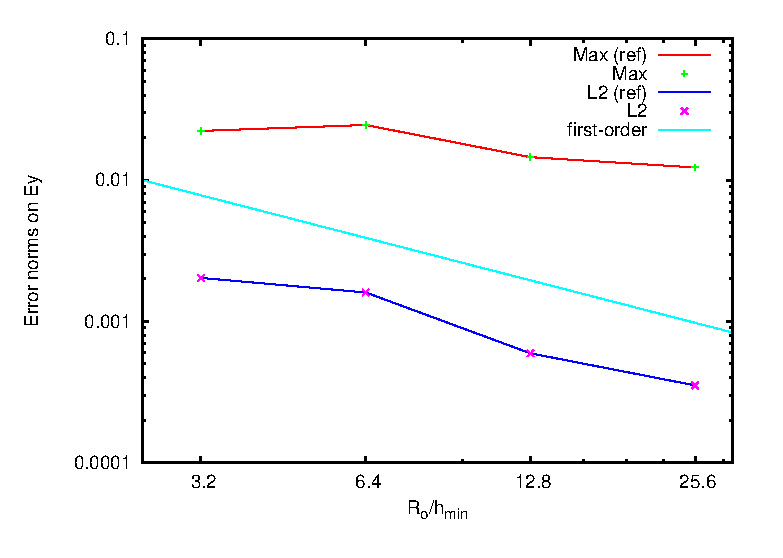
\includegraphics[width=\hsize]{source/error.eps}
\end{center}
\end{figure}

\begin{figure}[htbp]
\caption{\label{Relative Local Error} Local error at level 13. Color scale [-5e-4:5e-4].}
\begin{center}
\includegraphics[width=\hsize]{source/localerror.eps}
\end{center}
\end{figure}


\section{Axisymmetric}
\input{axi/axi.tex}
\input{axi/viscous/viscous.tex}
\input{axiadvection/axiadvection.tex}
\input{axiadvection/solid/solid.tex}

\section{Navier-Stokes}

\input{lid/lid.tex}
\input{lid/explicit/explicit.tex}
\input{poiseuille/poiseuille.tex}
\input{poiseuille/bagnold/bagnold.tex}
\input{couette/couette.tex}
\input{kinetic/kinetic.tex}
\input{hydrostatic/hydrostatic.tex}
\input{hydrostatic/quadratic/quadratic.tex}
\input{coriolis/coriolis.tex}

\section{Solid boundaries}

% command: boundaries.sh
% legend: Projection test of Almgren et al., 1997.

\begin{table}[htbp]
\begin{center}
\begin{tabular}{||l|c|c|c||c|c|c||} \hline
           & \multicolumn{3}{c||}{All cells} & \multicolumn{3}{c||}{Full 128 cells} \\ \hline
           & 128-256  & Rate & 256-512  & 128-256  & Rate & 256-512  \\ \hline
$L_1$      & 5.13e-04 & 1.60 & 1.69e-04 & 2.27e-04 & 1.87 & 6.23e-05 \\
$L_2$      & 2.78e-03 & 1.09 & 1.31e-03 & 4.74e-04 & 1.64 & 1.52e-04 \\
$L_\infty$ & 6.68e-02 & 0.59 & 4.44e-02 & 6.69e-03 & 0.38 & 5.13e-03 \\ \hline
\end{tabular}
\end{center}
\caption{Errors and convergence rates for the $x$-component of the velocity.}
\end{table}

\begin{table}[htbp]
\begin{center}
\begin{tabular}{||l|c|c|c||c|c|c||} \hline
           & \multicolumn{3}{c||}{All cells} & \multicolumn{3}{c||}{Full 128 cells} \\ \hline
           & 128-256  & Rate & 256-512  & 128-256  & Rate & 256-512  \\ \hline
$L_1$      & 4.47e-04 & 1.59 & 1.48e-04 & 2.31e-04 & 1.83 & 6.48e-05 \\
$L_2$      & 2.18e-03 & 1.11 & 1.01e-03 & 5.51e-04 & 1.68 & 1.72e-04 \\
$L_\infty$ & 4.87e-02 & -0.04 & 5.01e-02 & 8.69e-03 & 1.21 & 3.76e-03 \\ \hline
\end{tabular}
\end{center}
\caption{Errors and convergence rates for the $y$-component of the velocity.}
\end{table}

% command: channel.sh
% legend: Channel test of Almgren et al., 1997.

\begin{table}[htbp]
\begin{center}
\begin{tabular}{||l|c|c|c||c|c|c||} \hline
           & \multicolumn{3}{c||}{All cells} & \multicolumn{3}{c||}{Full 128 cells} \\ \hline
           & 128-256  & Rate & 256-512  & 128-256  & Rate & 256-512  \\ \hline
$L_1$      & 1.66e-04 & 1.21 & 7.18e-05 & 1.43e-04 & 1.49 & 5.08e-05 \\
$L_2$      & 3.77e-04 & 0.87 & 2.06e-04 & 3.29e-04 & 1.14 & 1.49e-04 \\
$L_\infty$ & 2.89e-03 & 0.52 & 2.01e-03 & 2.89e-03 & 0.52 & 2.01e-03 \\ \hline
\end{tabular}
\end{center}
\caption{Errors and convergence rates for the $x$-component of the velocity.}
\end{table}

\begin{table}[htbp]
\begin{center}
\begin{tabular}{||l|c|c|c||c|c|c||} \hline
           & \multicolumn{3}{c||}{All cells} & \multicolumn{3}{c||}{Full 128 cells} \\ \hline
           & 128-256  & Rate & 256-512  & 128-256  & Rate & 256-512  \\ \hline
$L_1$      & 7.34e-05 & 1.54 & 2.52e-05 & 5.73e-05 & 1.58 & 1.91e-05 \\
$L_2$      & 1.83e-04 & 1.39 & 6.99e-05 & 1.28e-04 & 1.53 & 4.44e-05 \\
$L_\infty$ & 1.65e-03 & 0.97 & 8.44e-04 & 9.83e-04 & 1.13 & 4.48e-04 \\ \hline
\end{tabular}
\end{center}
\caption{Errors and convergence rates for the $y$-component of the velocity.}
\end{table}

\input{plate/plate.tex}

\section{Moving solid boundaries}

\input{hexagon/hexagon.tex}
\input{strouhal/strouhal.tex}

\section{Surface tension}

\input{spurious/spurious.tex}
\input{spurious/axi/axi.tex}
\input{capwave/capwave.tex}
\input{capwave/density/density.tex}
\input{capwave/air-water/air-water.tex}
\input{capwave/gravity/gravity.tex}
\input{oscillation/oscillation.tex}

\section{Shallow-water}

\input{geo/geo.tex}
\input{geo/beta/beta.tex}
\input{waves/waves.tex}
\input{waves/adaptive/adaptive.tex}
\input{nz/nz.tex}

\section{Saint-Venant}

\input{parabola/parabola.tex}

\section{General Orthogonal Coordinates}

\input{lonlat/lonlat.tex}
\input{lonlat/coriolis/coriolis.tex}
\input{cosine/cosine.tex}
\input{harmonic/harmonic.tex}
\input{gaussian/gaussian.tex}

\section{Electrohydrodynamics}

\input{planar/planar.tex}
\input{planar/solid/solid.tex}
\input{bump/bump.tex}
\input{cylinder/cylinder.tex}
\input{cylinder/planar/planar.tex}
\input{electro/electro.tex}

\bibliographystyle{plain}
\bibliography{tests}

\end{document}
